\documentclass[12pt]{scrartcl}

 

\usepackage{float}

\usepackage[utf8]{inputenc}

\usepackage[T1]{fontenc}

\usepackage{lmodern}

\usepackage[ngerman]{babel}

\usepackage{amsmath}

\usepackage{graphicx}


 

\title{Versuch MI1\\ Mikrowellen}

\author{Frederik Strothmann, Henrik Jürgens}

\date{\today}


\begin{document}


 %deckblatt erstellen

\maketitle
\tableofcontents
\newpage

%einleitung zu dem experiment

\section{Einleitung}

Ein System aus Mikrowellensender und verschiedenen Empfängern ermöglicht Untersuchungen verschiedener physikalischer Effekte an Mikrowellen. So sollen in diesem Versuch stehende Wellen vermessen werden, außerdem wird die Wirkung einer Wachs-Sammellinse oder eines Polfilters (parallele Metallstäbe) untersucht sowie die Reflexion
an einer Wachsplatte (Brewster-Winkel), die Totalreflexion zwischen einer Wachs-Luft-
Wachs-Schicht und die Drehung der Polarisationsebene durch
”optisch aktive“ Substanzen.
(Spiralfedern in einem Styroporträger)
%versuchsaufbau mit skizze

\section{Versuchsaufbau}

%wenn du tabellen einfügst dann schreib bitte anstatt [htpb] [H]. zusammen mit \usepackage{float} verrutscht dann garnichts mehr
\section{Versuchsdurchführung}


\subsection{Praktische Durchführung}
\textbf{Allgemeine Hinweise:}\\
Die Mikrowellensender werden mit einer Gleichspannung von ca. 10 bis 12 V versorgt.
\begin{enumerate}
\item Zunächst stellen wir den Sender und eine Metallplatte im Abstand von ca. 30 - 40 cm gegenüber auf und zwischen beide die Diode. Dadurch bildet sich eine stehende Welle, sodass wir durch Verschieben der Metallplatte die Wellenlänge messen können.
\item
Wir messen die Intensitätsverteilung senkrecht zur Strahlrichtung mit dem Hornempfänger, wobei uns eine Wachslinse zur Verfügung stand:
\begin{enumerate}
\item ohne Linse (Abstand Sender-Empfänger ca. 1,5 m)
\item mit Linse (Abstand Sender-Linse 0,5 m, Linse-Empfänger 1 m)
\end{enumerate}

\item Die Totalreflexion der Mikrowellen soll anhand des folgenden Versuchs untersucht werden:

%hier die Abbildung aus der Versuchsanleitung einfügen, footnote muss noch geschrieben werden.
\begin{figure}[htbp] 
  \centering
    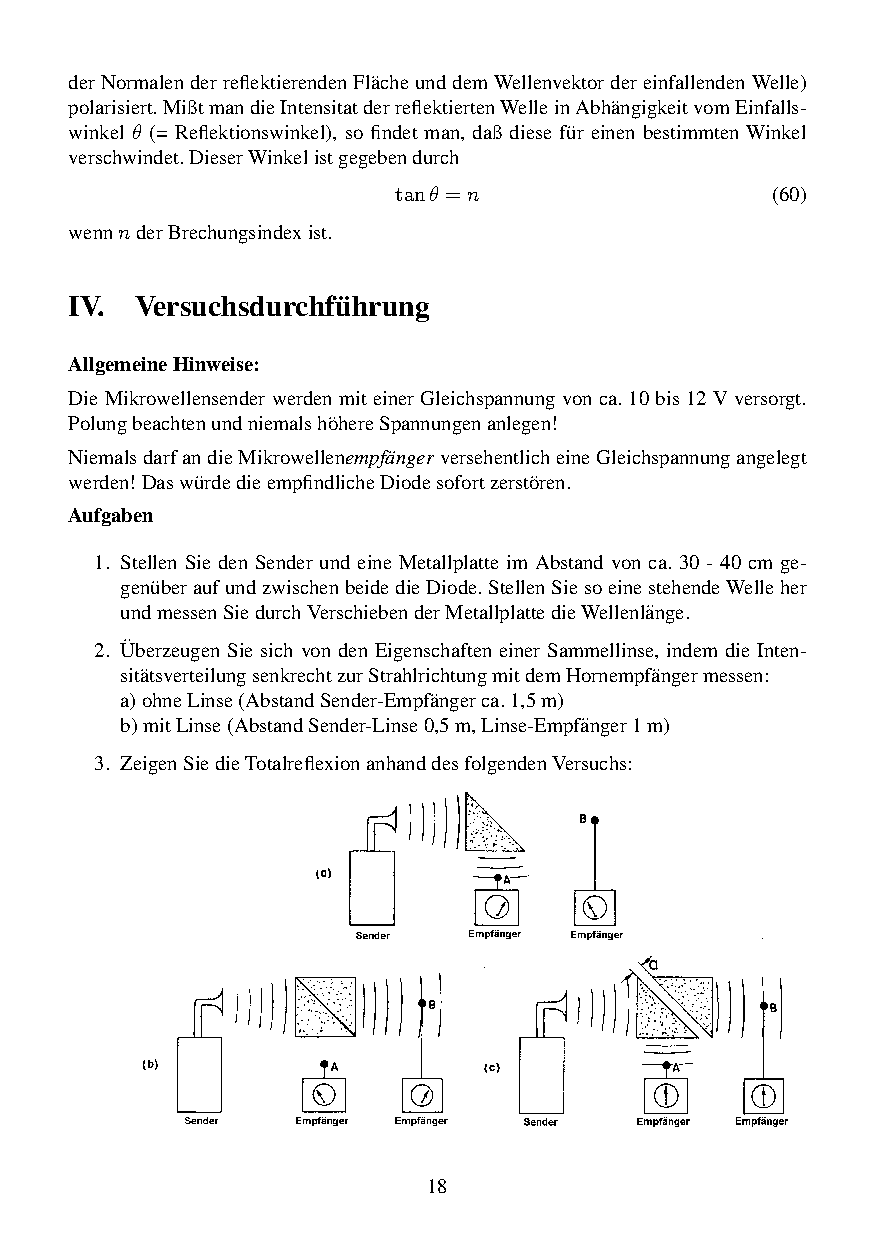
\includegraphics[trim = 80mm 15mm 0mm 160mm, clip, scale = 1]{totalreflexion.pdf}
  	\caption[Abbildung der beiden Schaltungen, für die Bestimmung des Wiederstandes]{Abbildung der beiden Schaltungen, für die Bestimmung des Wiederstandes\footnotemark}
  \label{fig:abb_versuch_3}
\end{figure}
\footnotetext{Abbildung entnommen von http://www.atlas.uni-wuppertal.de/~kind/MI1.pdf Seite 18 am 16.08.2014}

Die Wachsprismen werden ( n = 1,5 ) wie in Abbildung (c) gezeichnet im Abstand a gegenüber gestellt. Wir messen nun die Intensität des Empfängers in Abhängigkeit des Abstandes a.
%Versuchen Sie, die Erscheinung zu erklären.
\item In dieser Aufgabe stellen wir Sender und Empfänger  so gegenüber, dass die Polarisationsrichtungen (Richtungen, in denen der E-Vektor schwingt) der beiden parallel sind. Im Folgenden drehen wir den Empfänger um die Verbindungslinie von Sender und Empfänger und messen die Intensität in Abhängigkeit des Drehwinkels.

\item Sender und Empfänger nun um 90$^{\circ}$ gedreht gegenüber gestellt. Ein Gitter wird so zwischen Sender und Empfänger gehalten, dass die Stäbe mit dem E-Vektor einen Winkel von 45$^{\circ}$ bilden. Wir messen dazu die Intensität mit und ohne Gitter.

\item Abhängig vom Einfallswinkel messen wir die Intensität der von einer Wachsplatte reflektierten Wellen, die parallel zur Einfallsebene polarisiert sind. Daraus bestimmen wir den Brechungsindex.

\item Wir wollen die Drehung der Polarisationsebene durch ”optisch aktive“ Substanzen untersuchen. Es gibt dazu optisch aktive mit Rechtsschraubenfedern besetzte Styroporplatten. Die Platten sind durch eine Markierung (R) an der Seite der Styroporplatten gekennzeichnet.
\end{enumerate}

\subsection{Theoretische Durchführung}

\begin{enumerate}
\item
\item
\item
\item
\item
\item
\item
\end{enumerate}

\section{Messergebnisse}



\section{Auswertung}

\subsection{Aufgabe 1}
In der ersten Aufgabe sollte die Wellenlänge des Senders bestimmt werden, dabei wurden drei verschiedene Positionen gemessen siehe Tabelle  % \ref einfügen
es ergab sich in Mittelwert von:

\begin{align*}
2,7 (\pm 0,2) cm
\end{align*}


Auf dem Sender war ein Wert von 2,8 cm für die Wellenlänge angegeben.

\subsection{Aufgabe 2}
In der zweiten Aufgabe sollte der Effekt einer Sammellinse überprüft werden.
Dafür wurden Sender und Empfänger in einem Abstand von 1,5 Metern zueinander aufgestellt und die Intensität entlang der Orthogonalen vermessen. Dies geschah einmal mit der Sammellinse dazwischen und einmal ohne. Für die Messung ohne Sammellinse ergab sich der folgende Plot (die Werte sind Tabelle %\ref einfügen 
).

\begin{figure}[H]
\centering
    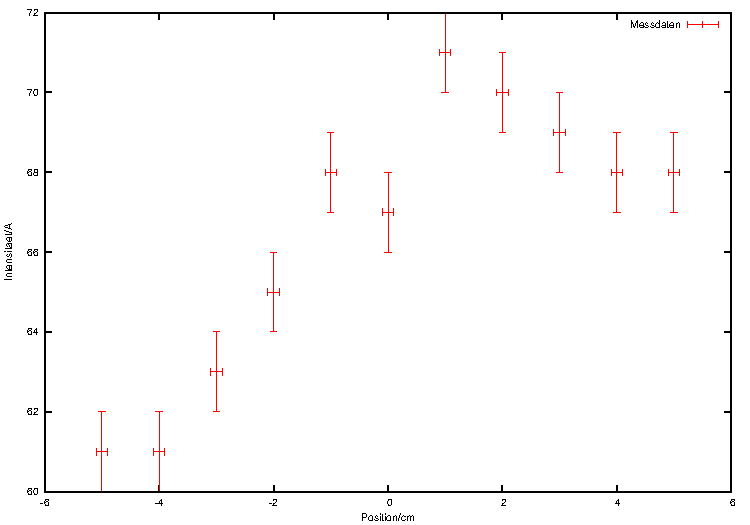
\includegraphics[scale = 1]{a_2_o.pdf}
  	\caption[Plot der Messung ohne Sammellinse]{Plot der Messung ohne Sammellinse}
  \label{fig:a_2_o}
\end{figure}

Bei der Messung mit Sammellinse ergab sich der folgende Plot (die Werte sind in Tabelle 
%\ref
).


\begin{figure}[H]
\centering
    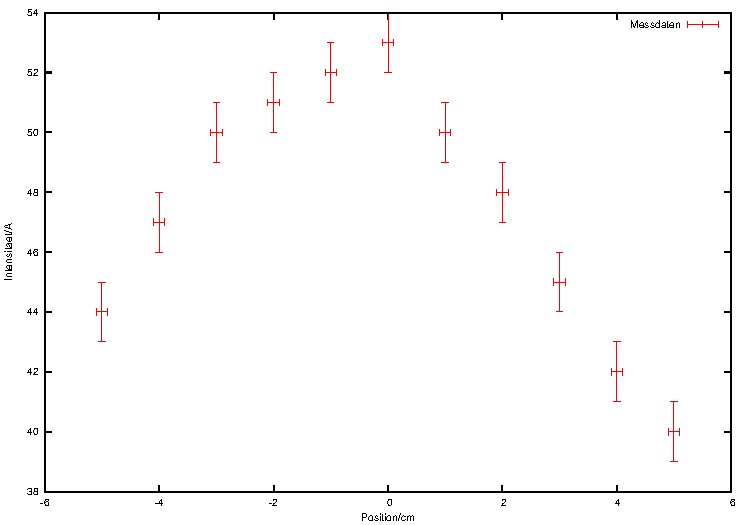
\includegraphics[scale = 1]{a_2_m.pdf}
  	\caption[Plot der Messung mit Sammellinse]{Plot der Messung mit Sammellinse}
  \label{fig:a_2_m}
\end{figure}
\section{Diskussion}


\subsection{Aufgabe 3}


 %Werte stimmen mit den Formeln überein/nicht überein

\end{document}

